%%% template.tex
%%%
%%% This LaTeX source document can be used as the basis for your technical
%%% paper or abstract. Regardless of the length of your document, the commands
%%% are all the same.
%%% 
%%% The "\documentclass" command is the first command in your file. If you want to 
%%% prepare a version of your article with line numbers - a "review" version - 
%%% include the "review" parameter:
%%%    \documentclass[review]{acmsiggraph}
%%%


\documentclass{acmsiggraph}

%%%packages to include
\usepackage{todonotes}
%%% Title of your article or abstract.

\title{Fused AR Experience}

\author{David~Dunn\thanks{e-mail:dunn@unc.edu}\\Abdul~Rafay~Khalid\thanks{e-mail:arkhalid@cs.unc.edu}} 
\pdfauthor{Abdul~Rafay~Khalid}

%%% Used by the ``review'' variation; the online ID will be printed on 
%%% every page of the content.

\TOGonlineid{45678}

% User-generated keywords.

\keywords{KinectFusion, RGBD, Augmented Reality}

% With the "\setcopyright" command the appropriate rights management text will be added
% to your document.

%\setcopyright{none}
%\setcopyright{acmcopyright}
%\setcopyright{acmlicensed}
\setcopyright{rightsretained}
%\setcopyright{usgov}
%\setcopyright{usgovmixed}
%\setcopyright{cagov}
%\setcopyright{cagovmixed}
%\setcopyright{rightsretained}

% The year of publication in the "\copyrightyear" command.

\copyrightyear{2016}

%%% Conference information, from the completed rights management form.
%%% The "\conferenceinfo" command has two parameters: 
%%%    - conference name
%%%    - conference date and location
%%% The "\isbn" field includes the year and month after the article ISBN.

\conferenceinfo{SIGGRAPH 2016 Posters}{July 24-28, 2016, Anaheim, CA} 
\isbn{978-1-4503-ABCD-E/16/07} 
\doi{http://doi.acm.org/10.1145/9999997.9999999}

\begin{document}

%%% This is the ``teaser'' command, which puts an figure, centered, below 
%%% the title and author information, and above the body of the content.

 \teaser{
   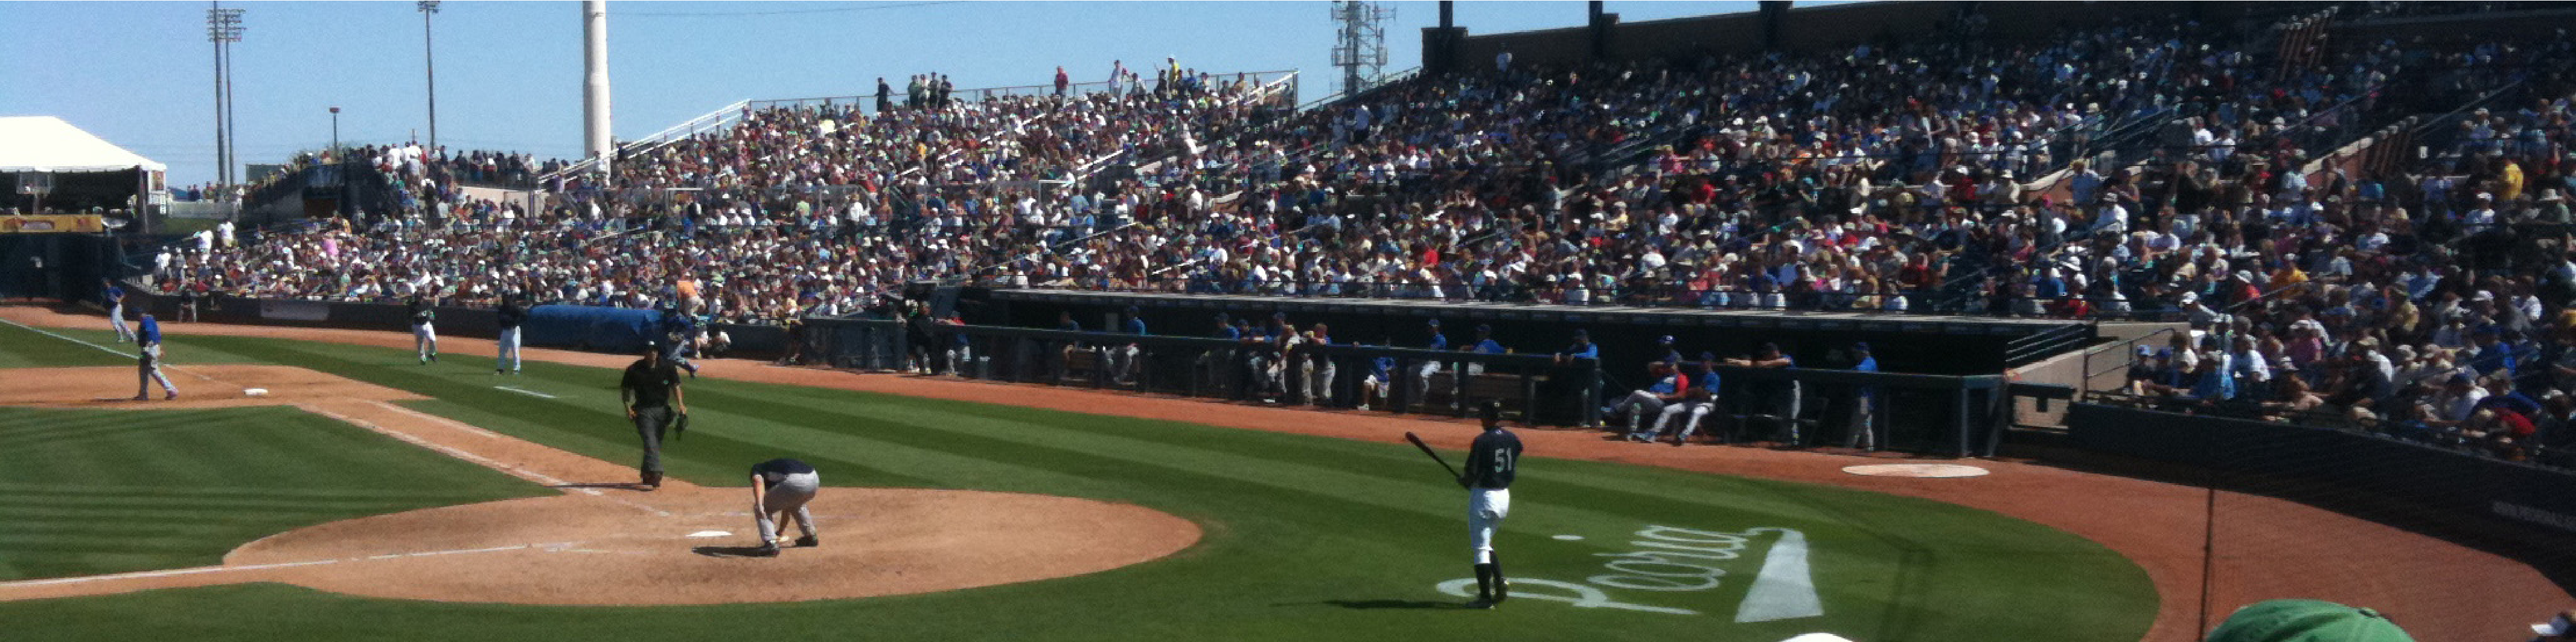
\includegraphics[height=1.5in]{images/sampleteaser}
   \caption{Spring Training 2009, Peoria, AZ.}
 }

\maketitle

\begin{abstract}
Traditionally Augmented Reality has taken three main forms each with its own drawbacks. Optical see-through gives us a good view of the real world but it is difficult to show virtual objects effectively as occlusion cannot be achieved. Spatial Augmented reality doesn't allow the user to view the virtual content at the correct depth. The closest to approach to ours is Video See through augmented reality however it suffers from mismatch between the location of eye and the camera center. In recent years there has been a lot of work on accurately reconstructing a 3D representation of the environment using RGBD sensors. We propose a system that combines such a realtime reconstruction method with a Head mounted display to create a wide field of view Augmnented Reality system. 

\end{abstract}

%
% The code below should be generated by the tool at
% http://dl.acm.org/ccs.cfm
% Please copy and paste the code instead of the example below. 
%
\begin{CCSXML}
<ccs2012>
<concept>
<concept_id>10010147.10010371.10010382</concept_id>
<concept_desc>Computing methodologies~Image manipulation</concept_desc>
<concept_significance>500</concept_significance>
</concept>
<concept>
<concept_id>10010147.10010371.10010382.10010236</concept_id>
<concept_desc>Computing methodologies~Computational photography</concept_desc>
<concept_significance>300</concept_significance>
</concept>
</ccs2012>
\end{CCSXML}

\ccsdesc[500]{Computing methodologies~Image manipulation}
\ccsdesc[300]{Computing methodologies~Computational photography}

%
% End generated code
%

% The next three commands are required, and insert the user-generated keywords, 
% The CCS concepts list, and the rights management text.
% Please make sure there is a blank line between each of these three commands.

\keywordlist

\conceptlist

\printcopyright

\section{Introduction}


Recent advances in reconstruction methods means that we can create a 3D representation of an environment in real time. The ability of these methods lead us to imagine an alternate form of Augmented Reality. By attaching an RGBD sensor to a VR HMD we can reconstruct the environment around the user as he moves around in his environment. As we have a 3D model of the environment we can render the view from each of the user's eyes. This enables us to accurately reproduce the real environment of the user in stereo. Virtual content can then be composited over the model of the real environment. By using the tracking from the reconstruction method we can align the virtual content with the reconstruction. 

\begin{figure}[ht]
	\centering
	\includegraphics[width=3.0in]{images/ferrari_laferrari}
	\caption{Ferrari LaFerrari. Image courtesy Flickr user ``gfreeman23.''}
	\label{fig:ferrari}
\end{figure}




\section{Related Work}
Our work is most related to the idea presented by \cite{izadi2011kinectfusion} that KinectFusion can allow for more realistic "Geometry Aware" Augmented Reality where virtual objects could be overlaid on the reconstruction of the real world. In the past Depth Cameras have been used in spatial augmented  reality for overlaying the a mesh of the real world on the environment and modifying it through interaction \cite{wilson2010combining}.\\
Our generation of virtual content relies on deforming the virtual model. This is achieved through the use of dual quaternion blending \cite{kavan2008geometric}.

\section{System Design}
Our setup consists of a Kinect camera rigidly aligned to an Oculus Rift HMD (Figure  \todo[inline]{Add picture of rft and kinect} ). The kinect acquires RGBD images which as used as input to the KinectFusion algorithm. Using the RGBD images, KinectFusion estimates the camera pose and uses this to integrate the current depthmap into the reconstruction. Virtual content is generated by animating a rigged model of a virtual character. The reconstruction is rendered from the viewpoint of the eyes. The virtual content is then composited onto this. If the virtual content is transformed using the same tracking as the reconstruction then it remains aligned to the environment.The combination of the reconstruction and virtual content is then rendered onto the HMD. Figure \todo[inline]{Add system overview figure} shows the System Overview. 
\missingfigure{System Overview}
\missingfigure{Picture of Rift}


\subsection{Environment Capture}
In order to capture the environment, we rely on the KinectFusion\cite{newcombe2011kinectfusion}  algorithm as our environment is static and we require the algorithm to be realtime. There are two main implementations of KinectFusion available. The Kinect Development Toolkit for Windows comes with an API to access KinectFusion. They do not provide source code but let the developer access KinectFusion in a limited matter. Also this version has only been demonstrated on small volumes and the tracking is not very stable when using large volumes with small voxel denisty. Given a camera pose and a camera matrix, the API allows the user to render the scene from that camera.\\
\begin{figure}[ht]
	\centering
	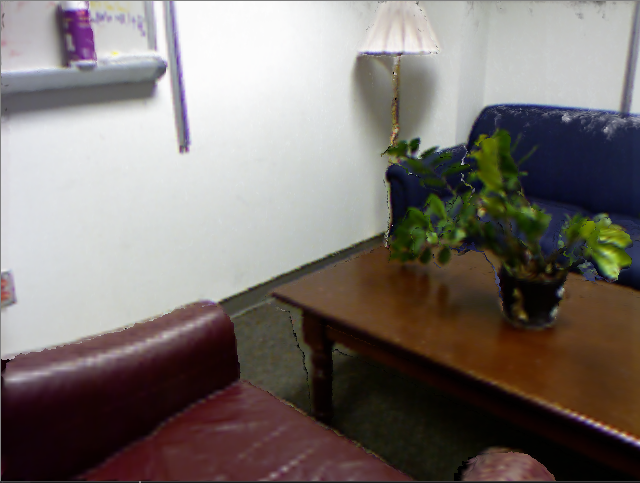
\includegraphics[width=3.0in]{images/scene2.png}
	\caption{A scene capture from Kinect}
	\label{fig:kinectFusionOut}
\end{figure}
The other popular implementation is KinFu that comes with PCL. This contains extensions on KinectFusion that enable it to work in large areas. It does so by decomposing the environment into chunks that can be uploaded to the GPU. This allows it to reconstruct a large volume while maintaining a high voxel density.This results in more robust tracking.  


\subsection{Generate Virtual Content}

\subsection{Composit Real and Virtuals}

\subsection{Tracking}

\subsection{Display on HMD}
\section{System Implementation}
As the KinFu implementation is open source and offers the ability to capture larger environments, we tried to use that first. KinFu comes in aversion of PCL that does not come with compiled binaries. Therefore we had to compile PCL from source. With some effort, we were able to get it to compile however there were certain dlls that PCL expected from Windows and those had changed in Windows 10 and so we were unable to run KinFu there. Observing this, we switched to Ubuntu. I was able to compile PCL on both my laptop and a machine obtained from the IT department. However, both machines failed to acknowledge the sensor. Eventually, it was found that our sensor even though the same model was slightly newer and was not supported by the OpenNI 1 library. OpenNI 2 that would've supported our sensor was not supported by KinFu. rather than waste anymore time on modifying KinFu source code to support OpenNI 2, we decided to abandon KinFu and switched to Microsoft's Kinect Fusion API. It gave us limited access to KinectFusion, in particular we could only rely on the API to render the the reconstruction for us. This also meant that we could only render content completely in front of the reconstruction and not partially occluded by it.
\section{Results}
As the user gets into our system, the world around him is reconstructed as he moves his head around. The user can walk around freely in this reconstructed environment as is tracked as he moves around. In addition to the reconstruction of the real world, he sees dynamic virtual characters that are aligned to the real world. Figure \todo[inline]{add image without virtual content} shows the experience without the virtual content and figure \todo[inline]{add image with virtual content} shows the experience with the virtual content.

\missingfigure{experience without virtual}

\missingfigure{Experience with virtual}
\section*{Acknowledgements}

To Robert, for all the bagels.

\bibliographystyle{acmsiggraph}
\nocite{*}
\bibliography{template}
\end{document}
